\chapter{Background}
\label{chp:background}

Section \ref{sec:bloppproject} will give a brief introduction to the history behind the BLOPP project. Section \ref{sec:about-asthma} will describe asthma and how it affects people. Section \ref{sec:cappgappkapp} will go into details of the applications that were developed by Aaberg, Aarseth, Dale, Gisvold and Svalestuen during the autumn of 2012.     
Section \ref{sec:existing-research} will give an introduction to some of the recent research that has been performed on mobile technology in combination with children and health.   


\section{BLOPP Project}
\label{sec:bloppproject}
The goal of the BLOPP project was to explore how design and technology can motivate children with respiratory diseases to take prescribed medication and to promote positive interactions between children and caregivers, thereby increasing adherence to medical treatment. BLOPP had previously worked with Asheim's ``Concept for improved treatment of children affected by asthma/RS-virus''\cite{asheim2012konsept} and H\o iseth's ``Research-Derived Guidelines for Designing Toddlers' Healthcare Games''\cite{hoiseth2013research}, in addition to several other projects.


\section{About Asthma}
\label{sec:about-asthma}
Asthma is a disease that affects the lungs. Asthma causes wheezing, breathlessness, chest tightness and coughing. It is a chronic disease, but asthma attacks will only occur when something is bothering the lungs. Asthma may be difficult to diagnose, especially in children under the age of five. 


An asthma attack may include coughing, chest tightness, wheezing and troubled breathing. The attack takes place in the lungs, the airways tighten which causes less oxygen to pass through.
According to the Norwegian Ministry of Health and Care Services, acute asthma attacks were the most common reason for hospitalization of children in 2008\cite{NationalStrategy}. In Norway, approximately 20 per cent of children are suffering from the disease. Due to this fact the condition may be said to have an effect on the economics of the society\footnote{Costs of having parents at home instead of working, hospitalization costs, medicine costs, etc.}. However, asthma can be controlled and asthma attacks avoided by taking medicine at regular intervals. Some of the medicines, such as Seretide and Flutide, are taken as a preventive measure to avoid asthma attacks. Ventoline is taken before exercise or when an asthma attack occurs, in order to stop or shorten the length of the attack. We will refer to this use as ``by need treatments''. 

A treatment may be done in different ways. For the youngest children a nebulizer is often used. The nebulizer is a device used to reduce liquid to an extremely fine cloud, in order to make it easier to inhale. Treatments using a nebulizer may last up to 10 or 15 minutes.

Older children use medication in spray or powder form (see Figure \ref{fig:inhalermask} and Figure \ref{fig:ventolinedisk} respectively). The spray is often used with a breathing chamber, and the powder form of medication is taken straight from the disk. Before use, the container of the asthma medicine must be shaken in order to stir the particles. If a breathing chamber is used, the protection cap is removed and the container is mounted on the breathing chamber. The chamber is pressed towards the user's face, covering the nose and mouth. The container is then pressed, to release the medicine into the breathing chamber, and the user breaths deeply for ten seconds\footnote{There are different ways to conduct a treatment. Some specialists advice to take six breaths instead of breathing for 10 seconds}. 

\begin{figure}[H]
	\begin{minipage}[b]{0.4\linewidth}
		\centering
			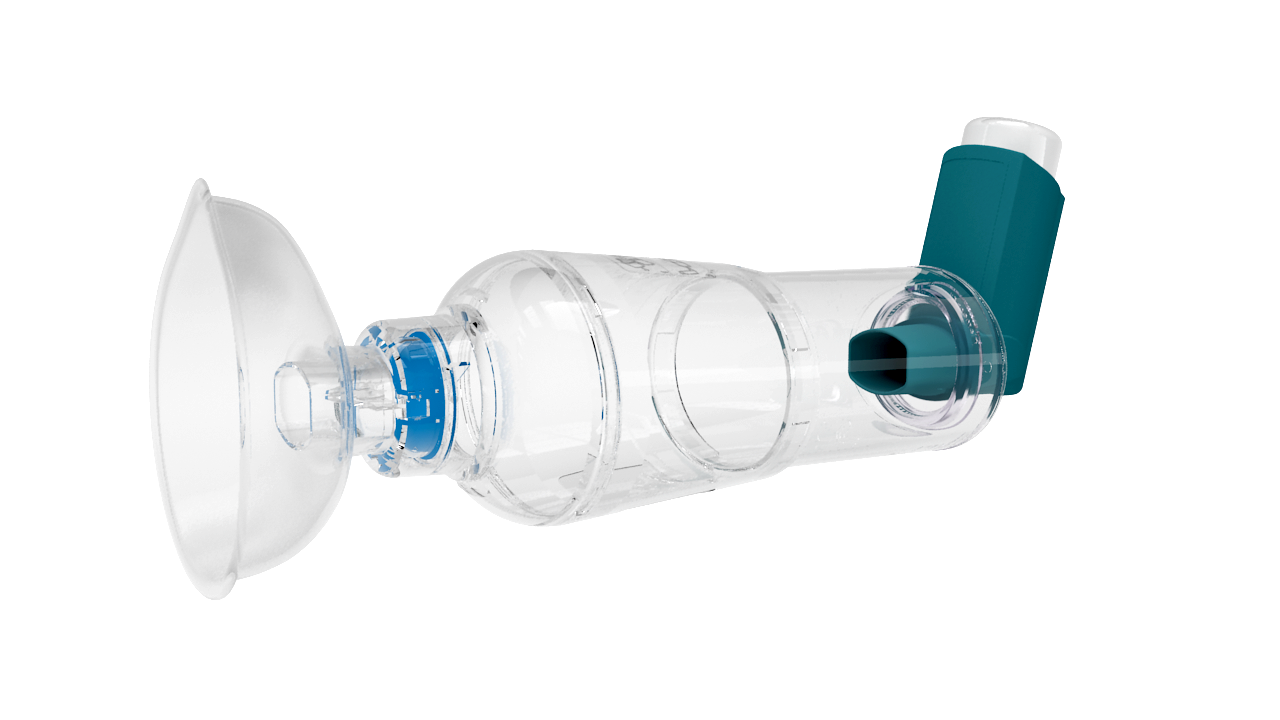
\includegraphics[width=0.20\paperwidth]{Pictures/asthmamask.png}
		\caption{\\ Breathing chamber with \\ inhaler mounted}
		\label{fig:inhalermask}
	\end{minipage}
	\hspace{3cm}
	\begin{minipage}[b]{0.4\linewidth}
		\centering
			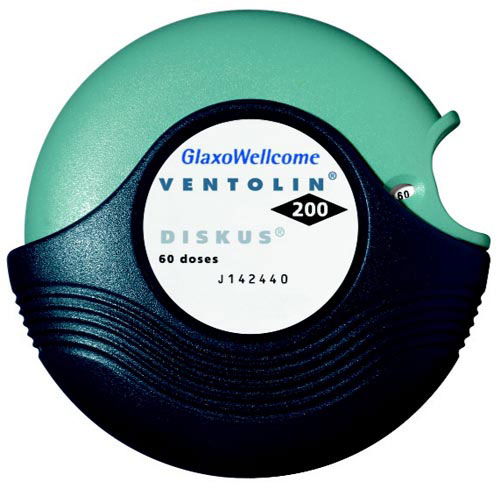
\includegraphics[width=0.20\paperwidth]{Pictures/ventolin.jpg}
		\caption{Ventoline in disk form}
		\label{fig:ventolinedisk}
	\end{minipage}
\end{figure}


\subsection{Ways Asthma Affect the Family}
\label{sec:waysasthmaaffectthefamily}
Before sending children to school or kindergarten, remembering to give the child his/her medication may prove challenging for the parents. Often the child does not enjoy taking his/her medicine, and the child may start an argument, not wanting to finish the treatment. This may result in parents applying the medication incorrectly, applying the wrong treatment, or even forgetting to give the medicine, which in turn may have a negative effect on the overall treatment.  

People suffering from asthma are often given an asthma control plan, which tells them how often they should take their medication and what to do if an attack occurs. These plans are often parted into three separate health zones, corresponding with how the user is feeling. In order to make these health zones understandable, an asthma action plan is often represented by a traffic light system (see Appendix \ref{chp:traffic-light}). The green treatment plan tells what the user should do when he/she has no symptoms. The yellow treatment plan indicates what to do when the user is feeling a bit ill, when there is a lot of pollen in the air or otherwise poor air quality or when the user is recovering from a cold. The red treatment plan indicates what to do when the user is feeling ill, or there is an extreme amount of pollen in the air or extremely poor air quality. If the red treatment plan is necessary, the child often has to consult a doctor. 

\section{CAPP, KAPP and GAPP}
\label{sec:cappgappkapp}
In the autumn of 2012 Aaberg, Aarseth, Dale, Gisvold and Svalestuen were engaged by the BLOPP Project group through the course ``TDT4290 - Customer Driven Project'' at NTNU\fnurl{Course Description of TDT4290 - Customer Driven Project}{http://www.idi.ntnu.no/emner/tdt4290/}. During the period of August 2012 to December 2012 they developed a prototype of a mobile information system consisting of two Android applications and a TUI. One application was developed for guardians of a child (GAPP) and the other for children (CAPP). Additionally, they created a Karotz application (KAPP) targeted at children\footnote{The creative process concerning the name of the applications were unfortunatly not prioritized}. In this section, we describe these applications, while a full report of their work is available online\cite{CustomerDriven}. 

Their prototype was the basis for our work in this project. 


\subsection{CAPP}
\label{sec:description-capp}
CAPP is an Android application targeted at children. Its main purpose is to guide the child through the medication process. Figure \ref{fig:capp-main-menu} shows the main page of CAPP\footnote{All applications have Norwegian as their main language}.  
As the target group for the application is children below the age of 8, it is reasonable to assume that not all of them are able to read, and consequently this application consists mainly of pictures and animations. However, some text is necessary since the amount of pictures and animations needed to explain everything would be overwhelming.


In CAPP, it is possible to start a medication in one of two ways. A parent can either set alarms in GAPP (See Section \ref{sec:description-gapp}) for preventive medicines, or a child can access the medication process directly by pressing the Karotz showed in Figure \ref{fig:capp-main-menu}, which is the way to start a by-need-treatment. 


One of the objectives of CAPP is to introduce a gamification experience to the medication process. Accordingly, the child recieves a golden star in his/her treasure chest once the medicine had been taken. However, these stars could not be used for anything, they were solely for display.
  

By clicking the treasure chest, the child is able to see how many stars he/she has aquired. A screenshot showing the inside of the treasure chest is included in Figure \ref{fig:capp_stars} 


The last part of this application is an Information-section, where information as to how to take a medicine is available. A part of the functionality that has not been implemented is voice over for these instructions. Thus, a parent should be close by in order to read the information contained in this functionality.     
Figures \ref{fig:instructions-1} - \ref{fig:instructions-7} shows the information-part of this application.

%CAPP MAIN MENU


%CAPP STARS & START TREATMENT
\begin{figure}[H]
	\begin{minipage}[t]{0.3\linewidth}
		\centering
			\fbox{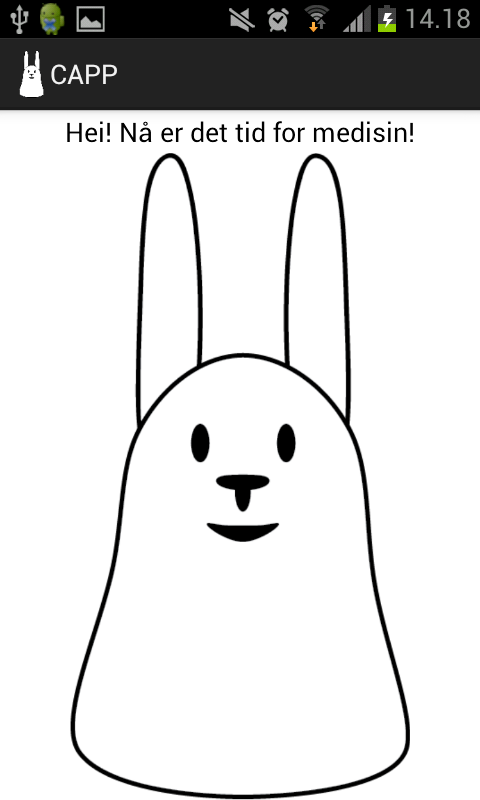
\includegraphics[width=0.20\paperwidth]{Pictures/app-screenshots/capp_start_treatment.png}}
		\caption{\\Starting a \\treatment}
		\label{fig:capp_start_treatment}
	\end{minipage}
	\begin{minipage}[t]{0.3\linewidth}
		\centering
			\fbox{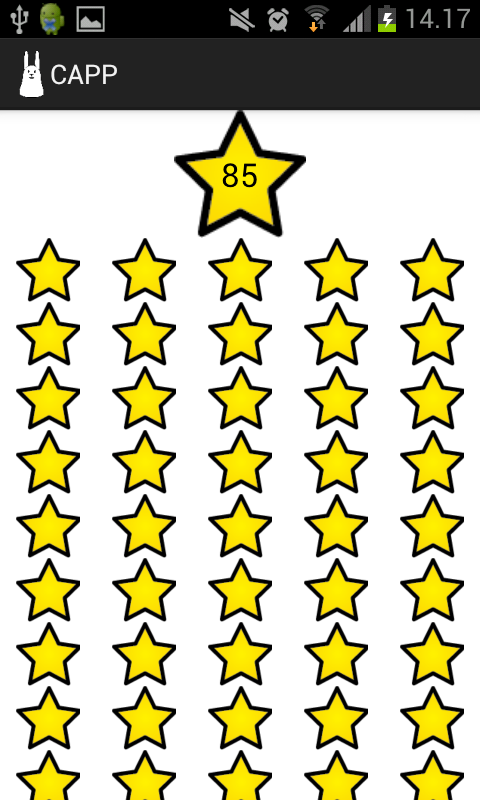
\includegraphics[width=0.20\paperwidth]{Pictures/app-screenshots/capp_stars.png}}
		\caption{Inside the treasure chest}
		\label{fig:capp_stars}
	\end{minipage}
	\begin{minipage}[t]{0.3\linewidth}	
		\centering
			\fbox{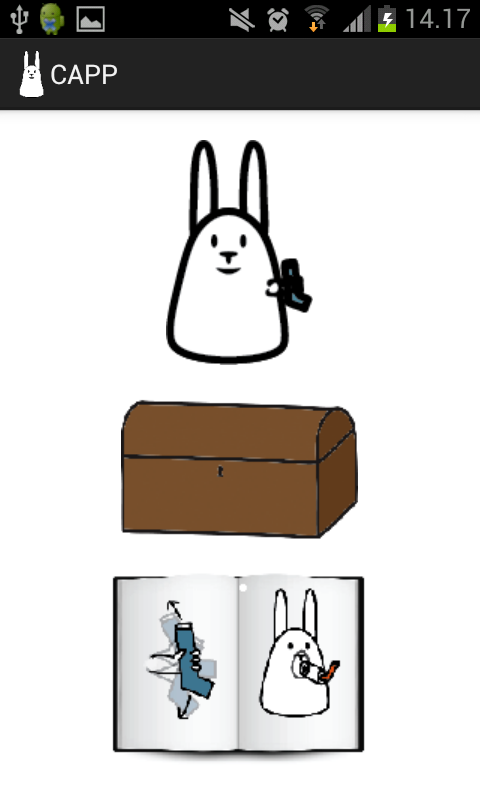
\includegraphics[width=0.20\paperwidth]{Pictures/app-screenshots/capp_main_menu.png}}
		\caption{CAPP main menu}
		\label{fig:capp-main-menu}
	\end{minipage} 
\end{figure}

%INSTRUKSJONER
\begin{figure}[H]
	\begin{minipage}[b]{0.3\linewidth}
		\centering
		\fbox{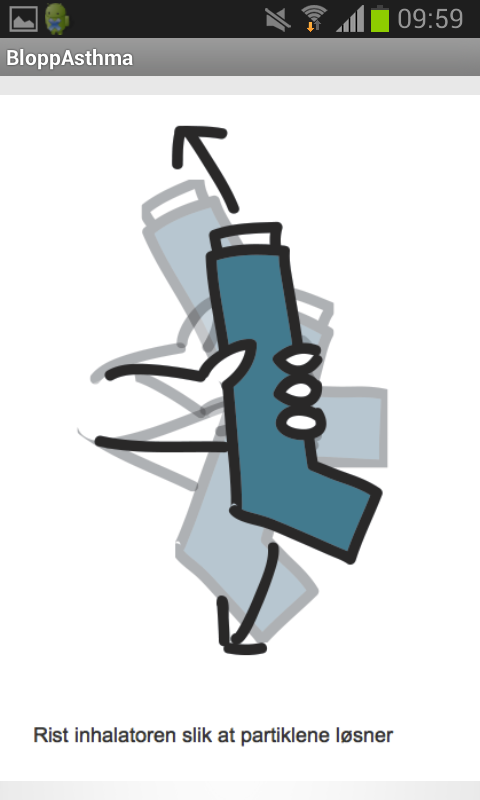
\includegraphics[width=0.20\paperwidth]{Pictures/app-screenshots/instructions-1.png}}
		\caption{\\ Instructions part 1}
		\label{fig:instructions-1}
	\end{minipage}
	\begin{minipage}[b]{0.3\linewidth}
		\centering
		\fbox{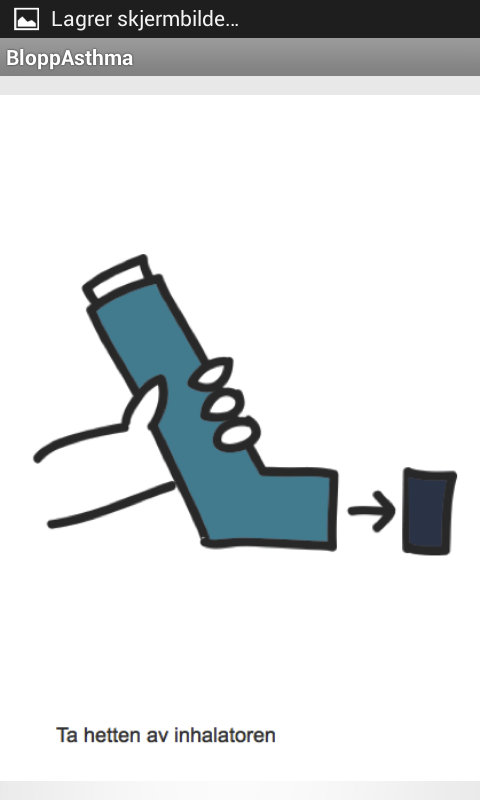
\includegraphics[width=0.20\paperwidth]{Pictures/app-screenshots/instructions-2.png}}
		\caption{\\ Instructions part 2}
		\label{fig:instructions-2}
	\end{minipage}
	\begin{minipage}[b]{0.3\linewidth}
		\centering
		\fbox{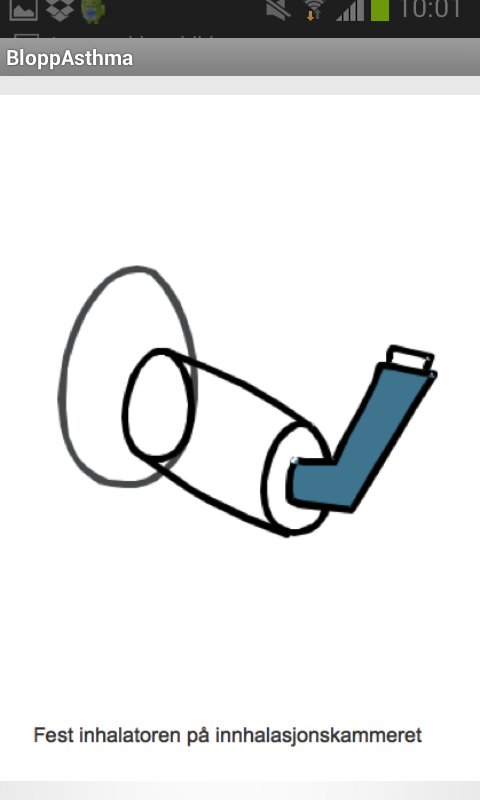
\includegraphics[width=0.20\paperwidth]{Pictures/app-screenshots/instructions-3.png}}
		\caption{\\ Instructions part 3}
		\label{fig:instructions-3}
	\end{minipage}
	
	\begin{minipage}[b]{0.3\linewidth}
		\centering
		\fbox{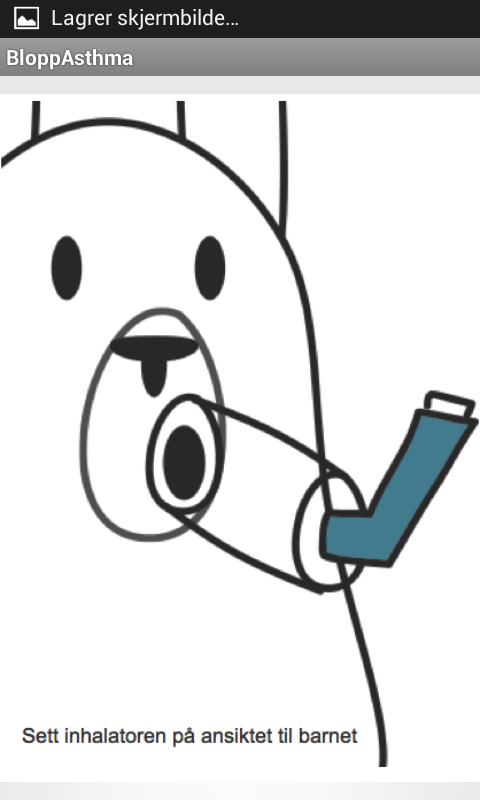
\includegraphics[width=0.20\paperwidth]{Pictures/app-screenshots/instructions-4.png}}
		\caption{\\ Instructions part 4}
		\label{fig:instructions-4}
	\end{minipage}
	\begin{minipage}[b]{0.3\linewidth}
		\centering
		\fbox{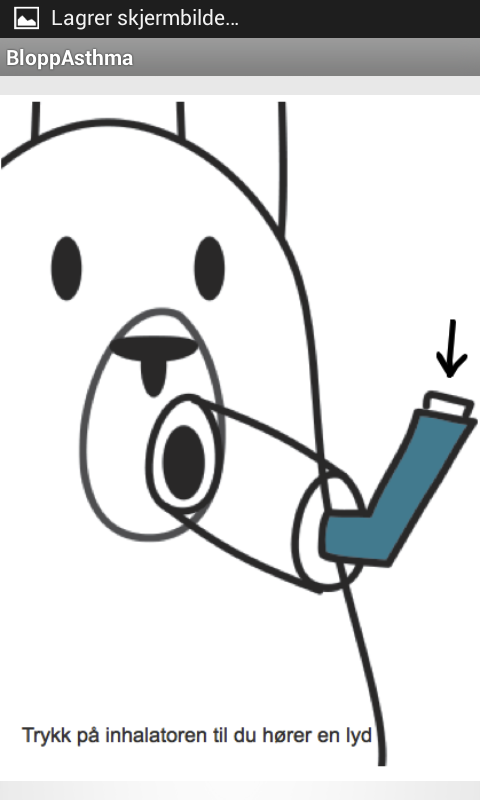
\includegraphics[width=0.20\paperwidth]{Pictures/app-screenshots/instructions-5.png}}
		\caption{\\ Instructions part 5}
		\label{fig:instructions-5}
	\end{minipage}
	\begin{minipage}[b]{0.3\linewidth}
		\centering
		\fbox{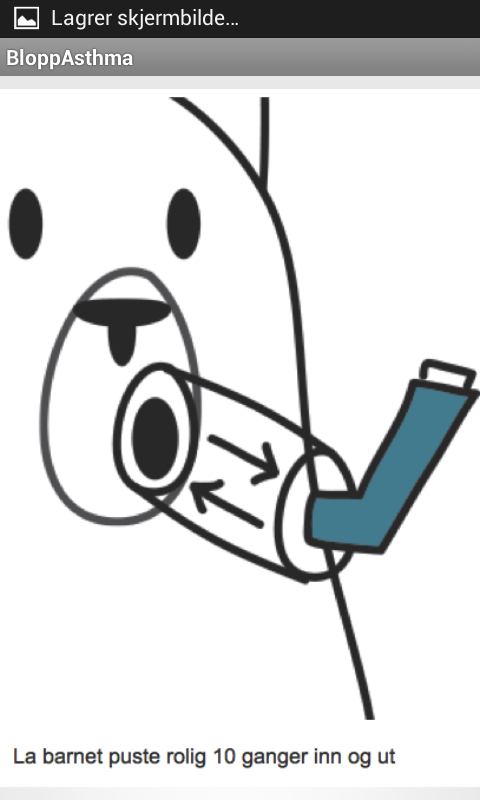
\includegraphics[width=0.20\paperwidth]{Pictures/app-screenshots/instructions-6.png}}
		\caption{\\ Instructions part 6}
		\label{fig:instructions-6}
	\end{minipage}
	
	\begin{minipage}[b]{0.3\linewidth}
		\centering
		\fbox{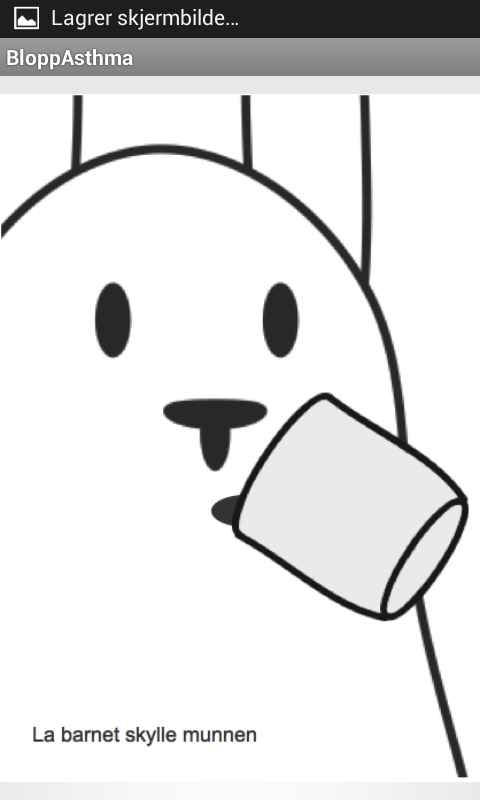
\includegraphics[width=0.20\paperwidth]{Pictures/app-screenshots/instructions-7.png}}
		\caption{\\ Instructions part 7}
		\label{fig:instructions-7}
	\end{minipage}
\end{figure}


\subsection{KAPP}
\label{sec:description-kapp}
KAPP is the TUI-application targeted at children. The application runs on a Karotz\fnurl{Karotz}{www.karotz.com}, which is a small robot bunny (see Figure \ref{fig:karotz}). The purpose of KAPP is similar to CAPP, namely to remind children when it is time to take the asthma medicine and give instructions during treatment. In order to interact with the Karotz, the child may use either a Nanoz (a small bunny with an integrated RFID) or by pressing a button on the top of the Karotz' head. It is not possible to do a by-need treatment with a Karotz as a companion. 


\begin{figure}[H]
	\begin{minipage}[b]{0.4\linewidth}
		\centering
			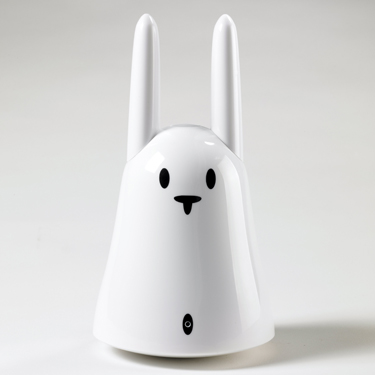
\includegraphics[width=0.20\paperwidth]{Pictures/karotz.jpg}
		\caption{Karotz}
		\caption*{Image source: Karotz \url{http://karotz.com}}
		\label{fig:karotz}
	\end{minipage}
	\hspace{3cm}
		\begin{minipage}[b]{0.4\linewidth}
		\centering
			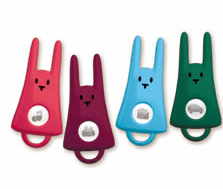
\includegraphics[width=0.20\paperwidth]{Pictures/app-screenshots/nanoz.png}
		\caption{Nanoz}
		\caption*{Image source: Karotz \url{http://karotz.com}}
		\label{fig:karotz}
	\end{minipage}
\end{figure}


\subsection{GAPP}
\label{sec:description-gapp}
GAPP is an Android application targeted at the guardians or parents of the child. 
Some parents have problems with remembering how often their child has taken his/her medication the last couple of days, when the child should take the medication and how the child's disease has evolved over a period of time. Thus, GAPP's main purpose is to make parents more aware of their child's disease.   


Figure \ref{fig:gapp-main-menu1} shows a screenshot of the main menu of GAPP. The main functionality is separated into 
\emph{Medical Plan}, \emph{Register Treatment}, \emph{Medicine Log}, \emph{Medical Information} and \emph{Manual}. 

\textbf{Medical Plan}

\emph{Medical Plan} gives parents the option to set up reminders at particular times. It is divided according to the asthma action plan (See Appendix \ref{chp:traffic-light}). A child has three separate plans, to ensure that an alarm that is set on the \emph{Danger}-plan is not automatically set on the \emph{Doing Well}-plan\footnote{In \app{} the different plans were named ``Healthy'', ``A little ill'' and ``Sick''}.   

\textbf{Register Treatment}

The \emph{Register Treatment}-option gives parents the possibility to register a treatment that was carried out in case the child for some reason did not go through the process in CAPP or KAPP. This way, the child will be rewarded with stars accordingly. Figure \ref{fig:gapp-register-treatment} shows a screen shot of this process.  

\textbf{Medical Information}

\emph{Medical Information} gives general information about different medicines, what they do and what they are used for. The three medicines that are currently in the system is Flutide, Seretide and Ventoline. Figures \ref{fig:information-1} and \ref{fig:information-2} shows screenshots of this functionality.

\textbf{Medicine Log}

\emph{Medicine Log} shows how many times a child has taken his/her medicine the last months. Figure \ref{fig:medicine-log} shows a screen shot of this functionality. A red circle marks the current day. A child's health state is displayed by the Green/Yellow/Red bar at the top of each day. In the bottom left corner, it is possible to show how much medicine was taken on a given day.
In the bottom right corner, Aaberg et. al. intended to show the pollen distribution for a given day. However, the pollen distribution data is only available during spring and summer, and thus Aaberg et. al created an artificial pollen distribution for demonstration purposes. 

\textbf{Manual}

The purpose of the \emph{Manual} is to help ``newcomers'' to medicate their child. For instance, if a relative is watching a child with asthma, he/she could use the application as a reference on how to do the process. At the time being, the manual shows Figures \ref{fig:instructions-1} - \ref{fig:instructions-7}, i.e. the content is equal to information section of CAPP. 
        
\begin{figure}[H]
	\begin{minipage}[t]{0.3\linewidth}
	\centering
		\fbox{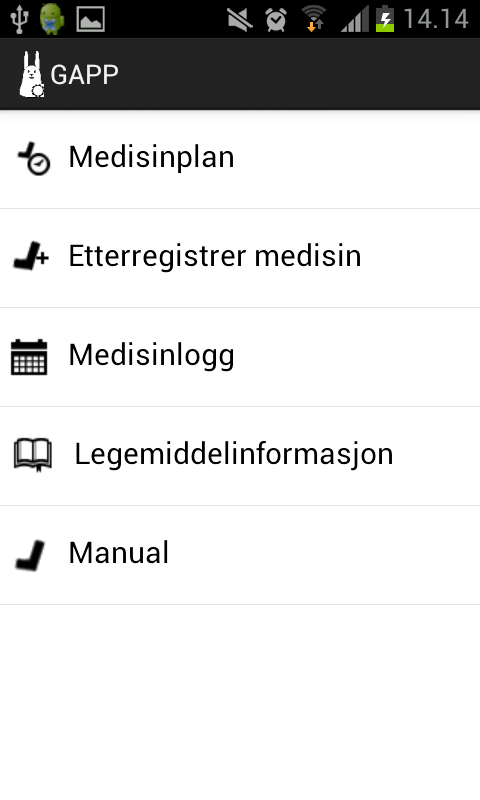
\includegraphics[width=0.20\paperwidth]{Pictures/app-screenshots/gapp_main_menu.png}}
		\caption{GAPP main menu}
		\label{fig:gapp-main-menu1}
	\end{minipage}
	\hspace{0.5cm}
	\begin{minipage}[t]{0.3\linewidth}
		\centering
		\fbox{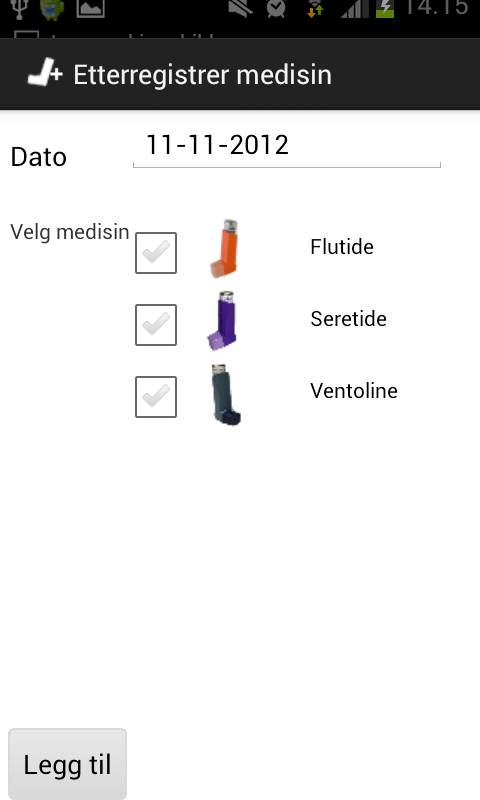
\includegraphics[width=0.20\paperwidth]{Pictures/app-screenshots/register_treatment_old.png}}
		\caption{\\ Register \\ treatment}
		\label{fig:gapp-register-treatment}
	\end{minipage}
	\hspace{0.5cm}
	\begin{minipage}[t]{0.3\linewidth}
		\centering
		\fbox{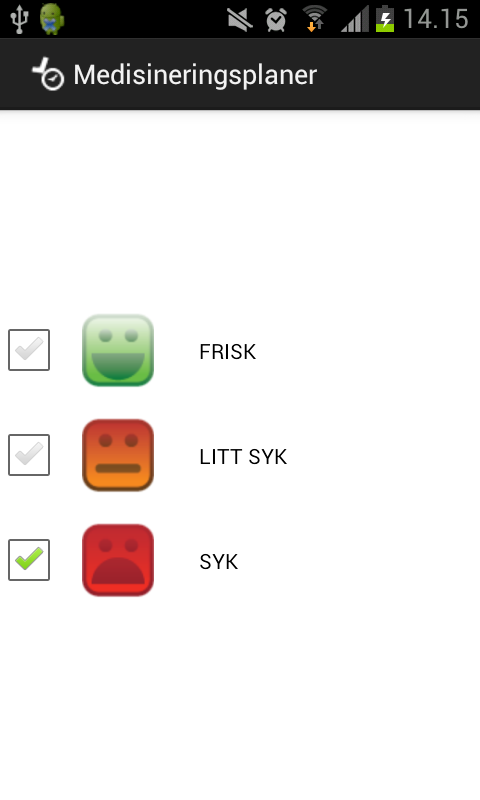
\includegraphics[width=0.20\paperwidth]{Pictures/app-screenshots/gapp_view_plans.png}}
		\caption{View plans}
		\label{fig:gapp-view-plans}
	\end{minipage}
\end{figure}

\begin{figure}[H]
\begin{minipage}[b]{0.3\linewidth}
		\centering
		\fbox{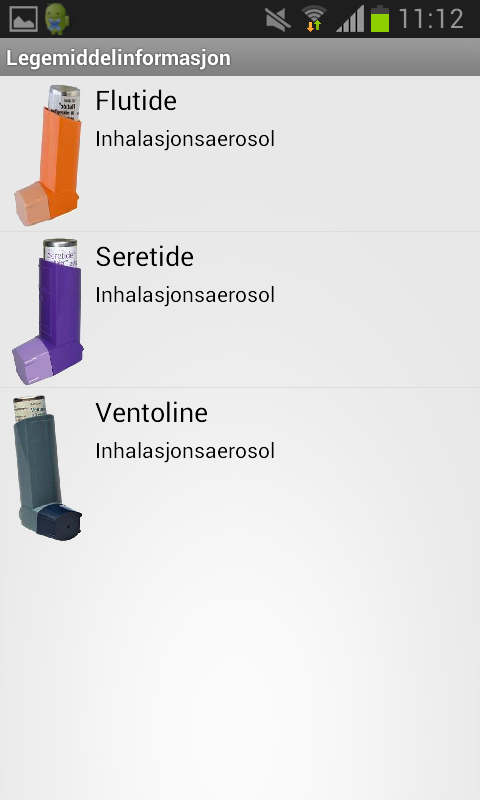
\includegraphics[width=0.20\paperwidth]{Pictures/app-screenshots/information-1.png}}
		\caption{\\ Information 1}
		\label{fig:information-1}
	\end{minipage}
	\hspace{0.5cm}
	\begin{minipage}[b]{0.3\linewidth}
		\centering
		\fbox{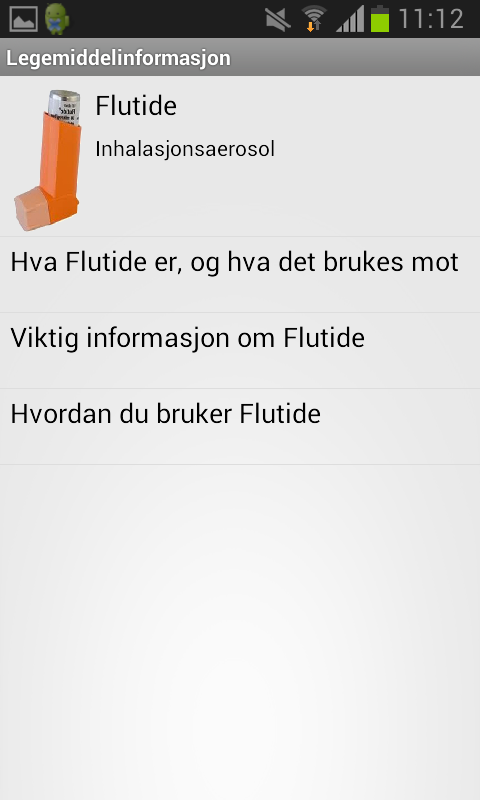
\includegraphics[width=0.20\paperwidth]{Pictures/app-screenshots/information-2.png}}
		\caption{\\ Information 2}
		\label{fig:information-2}
	\end{minipage}
	\hspace{0.5cm}
	\begin{minipage}[b]{0.3\linewidth}
		\centering
		\fbox{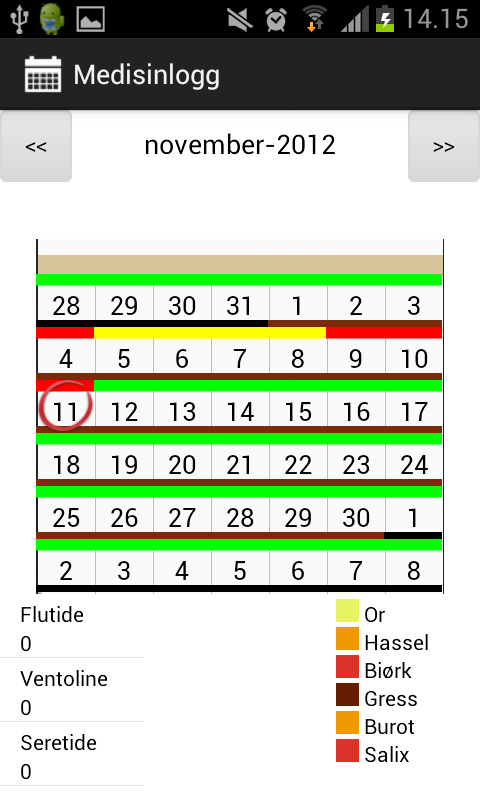
\includegraphics[width=0.20\paperwidth]{Pictures/app-screenshots/logg.png}}
		\caption{Medicine log}
		\label{fig:medicine-log}
	\end{minipage}
\end{figure}

\subsection{Known Areas For Improvement}
\label{sec:improvements}
As Aaberg \etal{} finished their work, they commented on several areas of potential improvement for CAPP, GAPP and KAPP. This document is reprinted in its entirety in Appendix \ref{app:furtherWork} (after permission from Aaberg, Aarseth, Dale, Gisvold and Svalestuen). The main topics for improvement were the reward system, the distraction sequence and a potential web application for storing, sending and visualizing data. 


These comments were used as a basis when we decided what to improve in this project. 

\section{Existing Research}
\label{sec:existing-research}

This section will give a foundation on some of the reserach performed on using technology in combination with diseases and children. 


\subsection{Monitoring Asthma with Mobile Technology}
There exists some research on self-management of monitoring your asthma condition. A lot of this research works used SMS (Short Messaging System) technology. In 2009, Andh\o j  et. al.\cite{anhoj2004feasibility} did a feasability study to check how users would respond to a SMS-reminder study. Their methodology was to send SMS a couple of times a day, and have the users respond to their peak flow and answer yes/no questions. Users could then access a web page to see different statistics on peak flows, how they've felt the last couple of days, etc.

They concluded that SMS is a feasible solution for collecting asthma diary data, mainly because the SMS technology was a big part of the participant's everyday life. Although SMS is a great technology to be used for this purpose, few children in our target group are able to use this technology, for obvious reasons. According to \emph{Senter for IKT i utdanningen} (Center for ICT in education), about 40\% of Norwegian children below the age of 3 years old have used a tablet, and 6 out of 10 children below the age of 6 have used a touch screen device \cite{nrkchilduse}. Thus the technological background should be somewhat familiar for our target group.  


\subsection{Children and Mobile Devices}
In 2013, \url{www.babies.co.uk} posted results on a poll they had posted on how many toddlers are using smartphones or tablets each day\cite{babiesusageoftablets}. Over 1000 participants responded,  and according to the survey, 14\% of the responders allowed children to use smartphones or tablets more than 4 hours a day. Considering the normal awake time of a child between 9 and 12 months old is approximately 10 hours, they spend a considerable amount of their day on the smartphone.         


\subsection{Children and Gestures}

Abdul Aziz et. al. \cite{aziz2013children} performed a study on which gestures children are able to comprehend when playing with an iPad. She tested 33 children's abililty to do gestures on a variety of applications suited for children. The children were in the range of 2-12 years old, 3 children per age. The study showed the following restrictions:

\begin{itemize}
  \item 2 year old children have difficulties with pinching, and are unable to drag and drop, spread and rotation of the device, and are not able to focus on the application. 
  \item 3 year old children have difficulties to drag and drop until they are told to do so, in addition to having problems with pinch and spread. 
  \item 4 year old children have difficulties to drag and drop. 
\end{itemize}
Children at age 5 and above are able to do all the normal gestures at a tablet. As CAPP is currently only available for mobile devices, this is reason for some discussion. The main part to notice is pinching and drag and drop. An iPad is fairly large relative to the size of these children's hands. There is reason to believe that gestures may be more difficult on smaller screens, however, we were unable to find research supporting this claim. In order to make AsthmAPP as child friendly as possible, it only uses ``swiping'' gestures and button presses for navigation.

\subsection{Assessment of Existing Applications}
In 2012, Huckvale et. al. \cite{huckvale2012apps} conducted an assesment on the existing applications on both Google Play\fnurl{Google Play}{http://play.google.com} and App Store\fnurl{Apple App Store}{http://www.apple.com/itunes/features}. They assessed 103 different apps with english as the native language. Out of these applications, 


\emph{``No apps for people with asthma combined reliable, comprehensive information about the condition with supportive tools for self­management''} \cite{huckvale2012apps}. 


They concluded that doctors should be careful when recommending apps for patients with the purpose of self management of asthma.

\section{State of the Art}
\label{sec:stateoftheart}
Mobile computing is evolving at a rapid pace, and finding new ways to use it in health care is a rising challenge for research. This section covers the state of the technological development of some of the areas in which mobile technology is being used with a combination of either gamification or tangible interfaces.   


\subsection{Get Up and Move (GUM)}
\label{sec:gum}
Penados et. al.\cite{penadosget} created GUM; an interactive toy to measure and stimulate physical activity. GUM is a small creature that needs to be taken care of by a child. The child's objective is to make his/her GUM healthier and happier by moving with it, feeding it and playing with it. GUM is healthy and happy when it has been through a minimal amount of daily physical activity, and since GUM can not move by itself, the child needs to do it. As GUM grows healthier, lighted stars will appear in its ears, until it reaches a maximum healthy state. To increase the number of stars, the child needs to progressively increase and later maintain the GUM's physical activity level. Penados et. al. argues that GUM had a positive effect on reducing sedentary behaviour and motivate physical activity with young children.


\subsection{Sisom}
\label{sec:sisom}
Sisom\fnurl{Sisom: Si det som det er}{http://www.communicaretools.org/sisom/} is a software created to increase the communication level between physicians and children. It is an interactive game, where the user follows an avatar through different ``worlds'' of health care subjects. For instance, the avatar takes a boat to a hospital. The user can look around in the hospital and express how he/she feels when giving a blood sample. The results showed that when a child played the game before a consultation with his/her physician, the child was better prepared, the communcication had a better quality, and the child participated more during the consultation\cite{sisom-research}.


\subsection{Meassuring Blood Pressure}
\label{sec:bloodpressure}
iHealth\fnurl{iHealth}{http://www.ihealthlabs.com/wireless-blood-pressure-monitor-feature\_32.htm}, Withings\fnurl{Withings}{http://www.withings.com/en/bloodpressuremonitor/features} and other companies has created blood pressure monitors which are synchronized with mobile applications. By using a wrist monitor; heartbeat, blood pressure level and pulse wave is meassured and stored in the application. The application visually presents graphs of the user's historic blood pressure levels and tracks progress. The application also allows for sharing meassurements with friends, family and doctors. By sharing detailed information with a doctor, a more accurate treatment plan may be laid out.


\subsection{Controlling Your Diabetes}
\label{sec:controldiabetes}
Cellnovo\fnurl{Cellnovo}{http://www.cellnovo.com/} has created a system that helps users to control their diabetes. It consists of a handheld device for meassuring blood sugar levels, a pump that controls the flow of insulin and a web interface that allows one to access the information. The interface helps users to check for trends and patterns in their blood sugar level, which again motivates users to continue applying the correct treatment. It also allows users to send information to physicians, which helps them make decisions regarding patient care.
      

\subsection{Quit Smoking}
\label{sec:quitsmoking}
There are lots of mobile applications that help people to quit smoking. For instance, \emph{The Norwegian Heart and Lung Patient Organization} has developed an app called ``'R\o ykeslutt''\fnurl{R\o ykeslutt}{https://play.google.com/store/apps/details?id=no.lhl.roykeslutt}. The application shows what the body is going through after a specific amount of days after the user has stopped smoking, which according to the reviews of the application, is a huge motivational factor. Additionally, they show how much money a user has saved at any given time, which can be seen as ``gamifying'' the element of money in order to motivate users.  


\subsection{TUIs and Multimodal Interfaces for Safety-Critical Applications}
Cohen \etal{} proposed the use of TUIs and Multimodal Interfaces(MMUI) for safety-critical applications \cite{cohen2004tangible}. They present an example with making strategic military planning of a battlefield. By combining special pens with cameras, CPUs and communication units, the lines drawn on a physical map would easily translate to a digital one. These tools made it easier to collaborate on making strategies and sharing them between officers. Cohen \etal{} argues that the combination of TUIs and MMUIs may make a suitable improvement for traditionally paper-heavy work.

\subsection{Exercise Games}
\label{sec:exercisegames}
In the last few years the exercise equipment industry has embraced gamification through their products. The use of experience points, badges, milestone goals and progress bars are commonly used to market products. Following are two, of many possible, examples of how the industry has made use of gamification. 

In 2012 Nike launched their Nike+ Fuelband\fnurl{Nike+ Fuelband}{https://secure-nikeplus.nike.com/plus/what\_is\_fuel/}, a wearable device for tracking the user's activity level. The Fuelband is worn as a bracelet, and has small LED lights indicating how active the user has been during the day. By being active the user collects NikeFuel\texttrademark, lighting more LED lights on the bracelet. The user may set goals for how active he/she should be in order to collect enough NikeFuel for the day. 

Nintendo Wii has gamified the way people exercise at home with Wii Fit and later Wii Fit Plus\fnurl{Wii Fit}{http://wiifit.com}. It gives a user the ability to choose his/her own training programme, including Yoga, Strength and Aerobics. The user can easily track his/her progress over several months. Additionally, it contributes to keeping children healthy, by having games that depend on the child's movement. For instance, if a child flaps his/her arms up and down, a bird on the screen is able to fly.
 
